\documentclass[a4paper]{article}
\usepackage{ulem}
\usepackage{setspace}
\usepackage{wrapfig}
\usepackage{bpchem}
\usepackage{color}
\usepackage{subfigure}
\usepackage{float}
\usepackage{titletoc}
\usepackage{indentfirst}
\usepackage{geometry}
\usepackage{amsmath}
\usepackage{amssymb}
\usepackage{graphicx}
\usepackage{enumerate}
\usepackage{url}
\usepackage{listings}
\usepackage{xcolor}
\lstset{
    numbers=left, 
    numberstyle= \tiny, 
    keywordstyle= \color{ blue!70},
    commentstyle= \color{red!50!green!50!blue!50}, 
    frame=shadowbox,
    rulesepcolor= \color{ red!20!green!20!blue!20} ,
    escapeinside=``,
    xleftmargin=2em,xrightmargin=2em, aboveskip=1em,
    framexleftmargin=2em
} 

\geometry{a4paper,left=2.5cm,right=2.5cm,top=2.5cm,bottom=2.5cm}

\begin {document}

\begin{large}
	\begin{center}
	~\\ ~\\ ~\\ ~\\ ~\\ ~\\ \rule[-1pt]{10.3cm}{0.05em} \\~\\UM-SJTU JOINT INSTITUTE\\~\\Probabilistic Methods in
Engineering\\~\\(VE401)	~\\ \rule[-1pt]{10.3cm}{0.05em} \vspace{7cm} \\Term Project 1
	\end{center}
\end{large}
~\\

\begin{large}
	\begin{center}
	Randomness and Pseudorandom Numbers
	\end{center}
\end{large}
\vspace{5cm}

\begin{tabular}{l l l}
	Name: Feitong Tang&ID: 518370910017&Group 1\\
	Name: Weikai Zhou&ID: 518021911039&Group 1\\
     ~\\
	Date: 3 April 2020
\end{tabular}


\newpage

\section{Abstract}
	This report shows some basic knowledge of pseudorandom numbers and pseudorandom number generators. It introduces basic ways of generating pseudorandom numbers, including linear congruential method and nonlinear congruential method. Moreover, it uses linear congruential method as an example to design a simple algorithm to generate pseudorandom numbers. After that, it also introduces some ways to test randomness such as monobit test, frequency test within a block and poker test. These tests are then applied to the generated pseudorandom numbers to test its randomness. Finally, it discusses some flaws in the pseudorandom number generator and randomness test.
\\

\noindent\textbf{Keywords}: pseudorandom numbers, pseudorandom number generators, randomness test.
	
\newpage

\tableofcontents

\newpage

\section{Introduction}
	\subsection{Background}
	Pseudorandom numbers are number sequences generated by certain computer algorithm that behave like random numbers. A pseudorandom number generator (PRNG) is the algorithm designed for producing numbers that can be regarded as random numbers. They are of great significance in our daily lives. They can be used in various aspects including simulations, electronic games and cryptography [1]. However, due to the limitations of algorithms, the numbers are not truly random, which may give people chances to predict the next number from the previous. Especially, the cryptographic applications need  almost perfect random numbers, otherwise, people can decode confidential information easily. Therefore, elaborate PRNGs are in demand nowadays.

	\subsection{Objectives}
	\begin{itemize}
	\item Understand some approaches that can be used to obtain pseudorandom numbers and choose one of them to create a feasible PRNG algorithm;
	\item Understand some approaches to testing the randomness of pseudorandom numbers and use them to test the randomness of the pseudorandom numbers generated by the PRNG algorithm;
	\item Identify some flaws of the PRNG.
	\end{itemize}


\section{Ways of obtaining pseudorandom numbers}
	There are different ways of obtaining pseudorandom numbers, and the project will basically introduce linear congruential method and nonlinear congruential method.

	\subsection{Linear congruential method}
	This is one of the most popular methods to generate pseudorandom numbers proposed by Lehmer in 1951. The general form of it can be written as $$x_{n+1} = \left( ax_n+c \right) {\rm mod}\,m.\eqno{(1)}$$ Here $\left\{ x_n \right\}$ is the sequence of pseudorandom numbers. $a$ is an integer greater than 1, known as the multiplier. $c$ is an integer known as the increment, and $m$ is the integer known as the modulus. And “$\left( ax_n+c \right) {\rm mod}\,m$” means the remainder of dividing $\left( ax_n+c \right)$ by $m$. The initial integer $x_0$ is known as the seed, and it is usually in the interval $\left[\,0,m\,\right)$. Therefore, all $x_n$ are in the interval $\left[\,0,m\,\right)$, and by dividing $m$, all $x_n$ can be mapped into the interval $\left[\,0,1\,\right)$ [2].

	Especially, if $c=0$, Eq. (1) can be written as $$x_{n+1} =  ax_n \, {\rm mod}\,m,\eqno{(2)}$$which is known as the multiplicative congruential generator. Besides, if $c\ne0$, people tend to call Eq. (1) mixed congruential generator [3].

	\subsection{Nonlinear congruential method}
	In 1981, Knuth proposed the nonlinear congruential generator. The general form of it can be written as $$x_{n+1}=(dx_n^2+ax_n+c)\,{\rm mod}\,m\quad(d\ne0).\eqno{(3)}$$ Here $\left\{ x_n \right\}$ is the sequence of pseudorandom numbers, and $m$ is the integer known as the modulus. In 1988, Eichenauer et al. came up with a more general form for nonlinear congruential generators $$x_{n+1}=f(x_n)\,{\rm mod}\,m, \eqno{(4)}$$ where the function $f(x_n)$ can be any functions other than linear function [2]. Also, by dividing $m$, all $x_n$ can be mapped into the interval $\left[\,0,1\,\right)$.


\section{A feasible PRNG algorithm}
	We are going to choose the linear congruential method as an example to create a feasible PRNG algorithm in C so that it can produce one hundred pseudorandom numbers in the interval $\left[\,0,100\,\right)$.

	\subsection{Designing process}
	As described in 3.1, we can let $a=2$, $c=3$. $m$ can be set as 100 since the interval of the pseudorandom numbers is $\left[\,0,100\,\right)$. Then an array that can store one hundred numbers is needed. For the starting point or the seed of the PRNG, the function “time(NULL)” provided by C can be used. It uses the current time to initialize “srand()”. Afterwards, the first pseudorandom number can be achieved with “x[0]=rand()\%100”. The “\%” here is like the function of “mod”, which can get the remainder. Furthermore, a “for-loop” should be used to repeat “x[i+1]=(a*x[i]+c)\%100” 99 times to get one hundred pseudorandom numbers. Finally, we can use “printf” to output all the numbers we get. The detailed code is attached in Appendix.
	
	\subsection{Demonstration and self-examination}
	With the code, we can run a test case. The pseudorandom numbers generated are listed in Table 1.

\begin{table}[H]
\centering
\begin{tabular}{|c|cccccccccccccccccccc|}
\hline
  & 1  & 2  & 3  & 4  & 5 & 6  & 7  & 8  & 9  & 10 & 11 & 12 & 13 & 14 & 15 & 16 & 17 & 18 & 19 & 20 \\ \hline
1 & 80 & 63 &    &    &   &    &    &    &    &    &    &    &    &    &    &    &    &    &    &    \\
2 & 29 & 61 & 25 & 53 & 9 & 21 & 45 & 93 & 89 & 81 & 65 & 33 & 69 & 41 & 85 & 73 & 49 & 1  & 5  & 13 \\
3 & 29 & 61 & 25 & 53 & 9 & 21 & 45 & 93 & 89 & 81 & 65 & 33 & 69 & 41 & 85 & 73 & 49 & 1  & 5  & 13 \\
4 & 29 & 61 & 25 & 53 & 9 & 21 & 45 & 93 & 89 & 81 & 65 & 33 & 69 & 41 & 85 & 73 & 49 & 1  & 5  & 13 \\
5 & 29 & 61 & 25 & 53 & 9 & 21 & 45 & 93 & 89 & 81 & 65 & 33 & 69 & 41 & 85 & 73 & 49 & 1  & 5  & 13 \\
6 & 29 & 61 & 25 & 53 & 9 & 21 & 45 & 93 & 89 & 81 & 65 & 33 & 69 & 41 & 85 & 73 & 49 & 1  &    &    \\ \hline
\end{tabular}
\caption{Pseudorandom numbers generated by the initial trial.}
\end{table}

	From this table, we can easily find that there is a loop in the numbers generated. The reason for this could be either the problem of x[0], or the problem of parameters $a$, $c$ and $m$. We test it again, and the new pseudorandom numbers also indicates the same loop as shown above. Therefore, the problem may be the value of $a$, $c$ and $m$. For example, if $m$ is small, then the values of remainders are limited, which increases the chance of falling into a loop like shown above. Hence, it is very important to choose appropriate values of $a$, $c$ and $m$. Some good values used by different platforms are listed in Appendix (Table 8).


	\subsection{Modification}
	Based on Table 8, we can re-design the algorithm. Let $m=134456$, $a=8121$ and $c=28411$. However, this will enlarge the interval of pseudorandom numbers to $[\,0,\,134456)$. In order to solve this problem, we can first map them into $[\,0,\,1)$ by dividing them with $134456$, and then re-map them into $[\,0,\,100)$ by timing them with 100. But the numbers we get now are not integers. We can use function “floor()” to round them, which will return the largest integer less than the value in the  brackets. The detailed code is attached in Appendix, and the pseudorandom numbers generated are listed below (Table 2).

\begin{table}[H]
\centering
\begin{tabular}{|c|cccccccccccccccccccc|}
\hline
  & 1  & 2  & 3  & 4  & 5  & 6  & 7  & 8  & 9  & 10 & 11 & 12 & 13 & 14 & 15 & 16 & 17 & 18 & 19 & 20 \\ \hline
1 & 13 & 79 & 56 & 25 & 82 & 86 & 1  & 36 & 90 & 98 & 65 & 19 & 47 & 40 & 38 & 67 & 90 & 42 & 79 & 16 \\
2 & 74 & 19 & 9  & 33 & 56 & 61 & 94 & 1  & 81 & 17 & 27 & 7  & 66 & 79 & 23 & 22 & 89 & 73 & 94 & 93 \\
3 & 73 & 38 & 42 & 27 & 69 & 18 & 43 & 75 & 47 & 42 & 31 & 16 & 79 & 15 & 85 & 50 & 22 & 99 & 15 & 76 \\
4 & 10 & 3  & 47 & 81 & 33 & 64 & 10 & 27 & 29 & 38 & 20 & 32 & 64 & 81 & 66 & 64 & 23 & 39 & 97 & 16 \\
5 & 89 & 28 & 6  & 1  & 37 & 27 & 18 & 33 & 12 & 57 & 74 & 14 & 22 & 72 & 14 & 19 & 16 & 40 & 71 & 82 \\ \hline
\end{tabular}
\caption{Pseudorandom numbers generated by the new code.}
\end{table}

	From Table 2, we may assume that there are no rules behind the numbers. However, in order to confirm this assumption, we need to find some ways that can test the randomness of the pseudorandom numbers.

\section{Ways of randomness test}

	Before turning to how to test randomness, we may first have a general idea of the level of randomness. Based on the research of National Institute of Standards and Technology (NIST), there are four ranks of randomness, which are represented as levels of security. For security level 1, which is the lowest one, it only requires the basic protection, while for level 3 and 4, they mainly focused on protecting information and are too complicated for only generating pseudorandom numbers [4]. Therefore, we will test the randomness of the given random sequence $x_1,x_2,...,x_n$ based on the second level of random numbers. According to the research papers of Bundesamt für Sicherheit in der Informationstechnik (BSI) and NIST, we will conduct the following tests [5][6]. (Some of them are used to test binary random sequences, so some modifications are made to fit our case.)
	
	\subsection{Monobit test}
	The monobit test is intended to test the frequency that each individual value appears. Thus, to make it simple and obvious, we will use the methods learned in class to conduct the test [5].
	
	We first calculate the theoretical expectation and then compare it to real mean. For the expectation and mean value, we have Eq. (5) and (6) respectively:
	
	$$E[X]=\sum\limits_{i=0}^{99}i\times\frac{1}{100}=49.5,\eqno{(5)}$$
	
	$$\overline{X}=\frac{1}{100}\sum\limits_{i=1}^{100}x_i.\eqno{(6)}$$
	
	If the relative error between these two values is less than $5\%$, we assume that the random sequence has passed the test. And a more obvious way is to draw the histogram and stem-and-leaf diagram and look at the plots' characteristics.
	
	\subsection{Frequency test within a block}
	
	This test divides the random sequence into $m$ non-overlapping blocks. Then we will count how many times each number inside the blocks appears. Since in our case the number ranges from 0 to 99, which is hard to focus on a specific value, we will test the frequency of intervals instead of a single number [6].
	
	For this test, we will divide the sequence into 5 blocks with 20 numbers each. Also, we will divide [0,100) to 5 subintervals, namely [0,19], [20,39], [44,59], [60,79], [80,99]. Then we will calculate the frequency that numbers in each block fall into the intervals. It is easy to see that theoretically, each interval will have about 4 numbers.
	
	If the actual result corresponds to the theoretical one, then the random sequence passes the test.
	
	\subsection{Poker test}
	Poker test is also a classical test for checking randomness. When carrying out Poker test, the random sequence is divided into $m$ non-overlapping subsequences with equal length. Then the pattern of each subsequence is studied, the appearing frequency of which should follow a chi-square distribution [5].
	
	In our case, we divide the random sequence into 10 subsequences with each subsequence having 10 numbers. However, it will be complicated to analyze the patterns of 10 numbers. Thus, we refer to an approximate poker test [7]. For the approximate poker test, we focused on the number of different values shown up rather than a specific kind of pattern. This will reduce the workload a lot. In the research paper, the probability with $r$ different values is shown as follow [7]:
	
	$$P=\frac{100!}{100^{10}\times(100-r)!}\begin{Bmatrix}10\\r\\ \end{Bmatrix},\eqno{(7)}$$
	where $\begin{Bmatrix}10\\r\\ \end{Bmatrix}$ is called the Stirling number, and it can be calculated as follows [8]:
	
	$$\begin{Bmatrix}n\\m\\ \end{Bmatrix}=\frac{1}{m!}\sum\limits_{k=0}^m(-1)^k\begin{pmatrix}m\\k\\ \end{pmatrix}(m-k)^n.\eqno{(8)}$$
	
	Then based on Eq. (7) and (8), we can get the following table (Table 3) describing the poker test probability. A sample calculation of $r=9$ is given:
	
	$$P=\frac{100!}{100^{10}\times(100-9)!}\begin{Bmatrix}10\\9\\ \end{Bmatrix}=\frac{100!}{100^{10}\times91!}\times\frac{1}{9!}\sum\limits_{k=0}^9(-1)^k\begin{pmatrix}9\\k\\ \end{pmatrix}(9-k)^{10}=0.311.\eqno{(9)}$$
	
	
	\begin{table}[H]
	\centering
	\begin{tabular}{|c|c|c|}
	\hline
	the number of different values&Stirling number&probability\\
	\hline
	1&1&$1\times10^{-18}$\\
	\hline
	2&511&$5.06\times10^{-14}$\\
	\hline
	3&9330&$9.05\times10^{-11}$\\
	\hline
	4&34105&$3.21\times10^{-8}$\\
	\hline
	5&42525&$3.84\times10^{-6}$\\
	\hline
	6&22827&$1.96\times10^{-4}$\\
	\hline
	7&5880&$4.74\times10^{-3}$\\
	\hline
	8&750&0.0563\\
	\hline
	9&45&0.311\\
	\hline
	10&1&0.628\\
	\hline
	\end{tabular}
	\caption{The Stirling numbers and the probability of subsequence with different numbers.}
	\end{table}
	
	Then based on the table, we can check whether the random sequence passes the poker test.	
	

\section{Tests for randomness of the PRNG}

\subsection{Monobit test}
	Based on Table 2, we can calculate the mean of the pseudorandom numbers:

	$$\overline{X}=\frac{1}{100}\sum\limits_{i=1}^{100}x_i=46.25.\eqno{(10)}$$	
	
	Thus, the relative error is 
	$$\frac{|49.5-46.25|}{49.5}=6.56\%.\eqno{(11)}$$
	
	Also, Figure 1 shows the histogram and stem-and-leaf diagram of the random sequence.
	
	\begin{figure}[H]
	\centering
	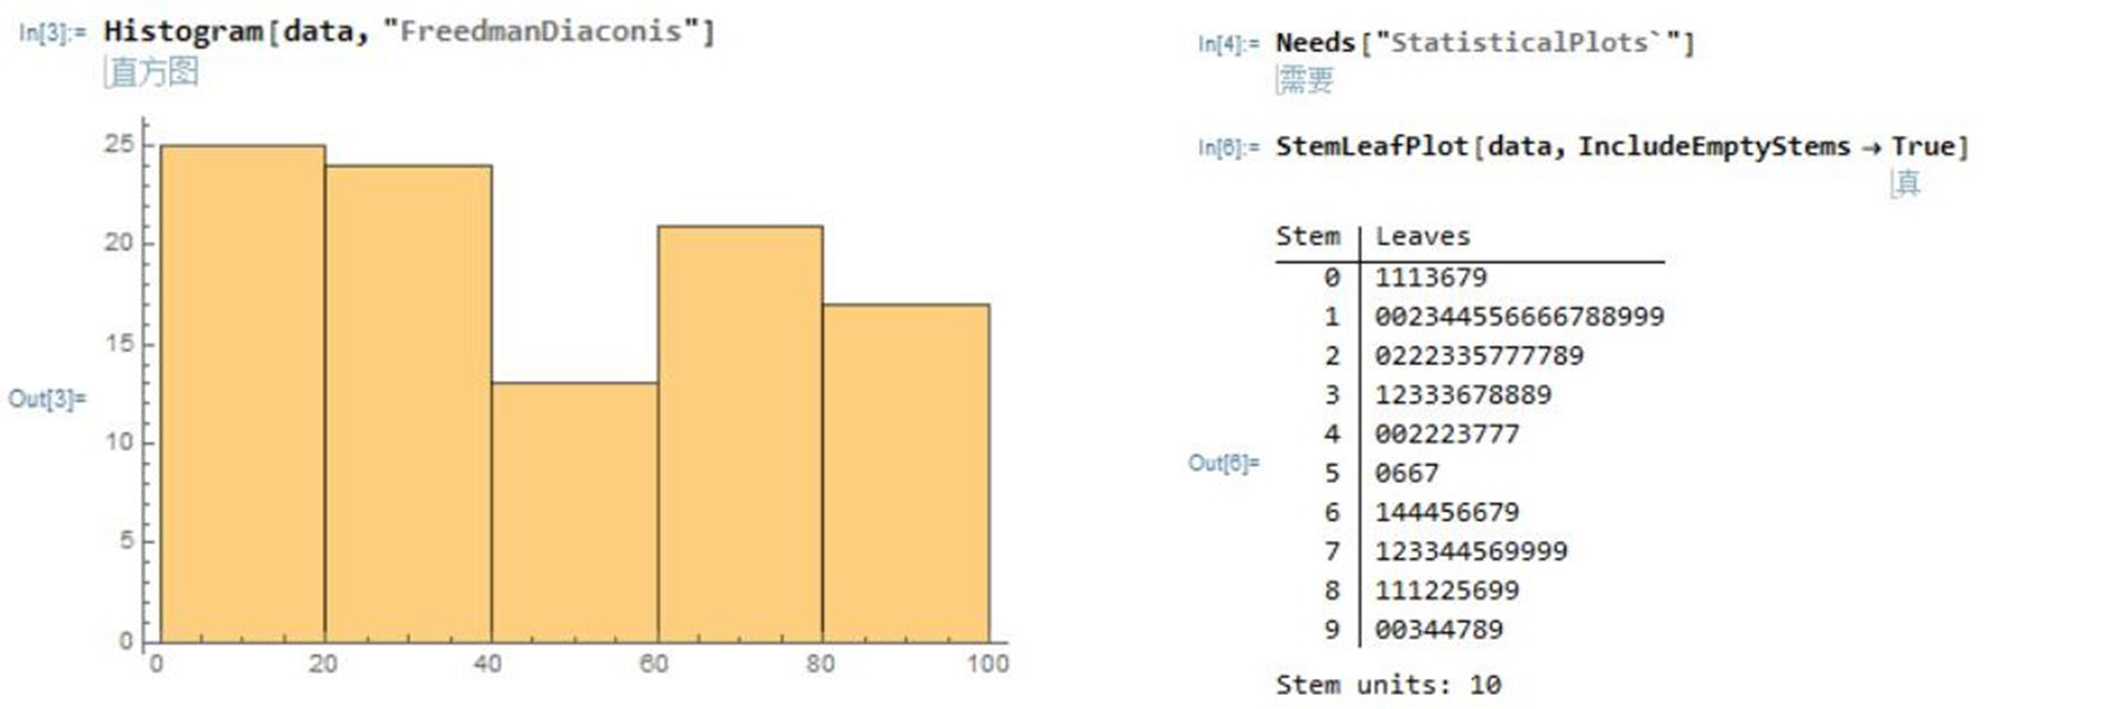
\includegraphics[height=7cm,width=18cm]{2.jpg}
	\caption{The histogram and stem-and-leaf diagram of random numbers.}
	\end{figure}
	
	From the diagrams, we can see that there are some unevenly distributed signs of the numbers. Therefore, we may doubt that the numbers generated has low randomness.
	
	\subsection{Frequency test within a block}
	We first divide the pseudorandom numbers into 5 blocks (Table 4).
	
	\begin{table}[H]
	\centering
	\begin{tabular}{|c||cccccccccccccccccccc|}
	\hline
block 1 & 13 & 79 & 56 & 25 & 82 & 86 & 1  & 36 & 90 & 98 & 65 & 19 & 47 & 40 & 38 & 67 & 90 & 42 & 79 & 16 \\	\hline
block 2 & 74 & 19 & 9  & 33 & 56 & 61 & 94 & 1  & 81 & 17 & 27 & 7  & 66 & 79 & 23 & 22 & 89 & 73 & 94 & 93 \\	\hline
block 3 & 73 & 38 & 42 & 27 & 69 & 18 & 43 & 75 & 47 & 42 & 31 & 16 & 79 & 15 & 85 & 50 & 22 & 99 & 15 & 76 \\	\hline
block 4 & 10 & 3  & 47 & 81 & 33 & 64 & 10 & 27 & 29 & 38 & 20 & 32 & 64 & 81 & 66 & 64 & 23 & 39 & 97 & 16 \\	\hline
block 5 & 89 & 28 & 6  & 1  & 37 & 27 & 18 & 33 & 12 & 57 & 74 & 14 & 22 & 72 & 14 & 19 & 16 & 40 & 71 & 82 \\ \hline
\end{tabular}
\caption{5 blocks of the random sequence.}
\end{table}
	
	Then the numbers in each block are divided into five intervals (Table 5).
	
	\begin{table}[H]
	\centering
	\begin{tabular}{|c|l|l|l|l|l|}
	\hline
	&[0,19]&[20,39]&[40,59]&[60,79]&[80,99]\\
	\hline
	block 1&13,1,19,16&25,36,38&56,47,40,42&79,65,67,79&82,86,90,98,90\\
	\hline
	block 2&19,9,1,17,7&33,27,23,22&56&74,61,66,79,73&94,81,89,94,93\\
	\hline
	block 3&18,16,15,15&38,27,31,22&42,43,47,42,50&73,69,75,79,76&85,99\\
	\hline
	block 4&10,3,10,16&33,27,29,38,20,32,23,39&47&64,64,66,64&81,81,97\\
	\hline
	block 5&6,1,18,12,14,14,19,16&28,37,27,33,22&57,40&74,72,71&89,82\\
	\hline
	
	\end{tabular}
	\caption{Result of frequency test within a block.}
	\end{table}		
	
	From Table 5, we see that the numbers in general are evenly distributed, but there are still some unexpected features. We can see the numbers in the interval [40,59] is less than average. This may be due to the limited length of random sequence, but also indicates the low randomness.
	
	\subsection{Poker test}
	
	We divide the sequence into 10 non-overlapping subsequences labeled as (1), (2), ..., (10) (Table 6).
	
	\begin{table}[H]
	\centering
	\begin{tabular}{|c|cccccccccc||c|cccccccccc|}
	\hline
(1) & 13 & 79 & 56 & 25 & 82 & 86 & 1  & 36 & 90 & 98&(2) & 65 & 19 & 47 & 40 & 38 & 67 & 90 & 42 & 79 & 16 \\	\hline
(3) & 74 & 19 & 9  & 33 & 56 & 61 & 94 & 1  & 81 & 17&(4) & 27 & 7  & 66 & 79 & 23 & 22 & 89 & 73 & 94 & 93 \\	\hline
(5) & 73 & 38 & 42 & 27 & 69 & 18 & 43 & 75 & 47 & 42 &(6)& 31 & 16 & 79 & 15 & 85 & 50 & 22 & 99 & 15 & 76 \\	\hline
(7) & 10 & 3  & 47 & 81 & 33 & 64 & 10 & 27 & 29 & 38&(8) & 20 & 32 & 64 & 81 & 66 & 64 & 23 & 39 & 97 & 16 \\	\hline
(9) & 89 & 28 & 6  & 1  & 37 & 27 & 18 & 33 & 12 & 57 &(10)& 74 & 14 & 22 & 72 & 14 & 19 & 16 & 40 & 71 & 82 \\ \hline
\end{tabular}
\caption{10 blocks of the random sequence.}
\end{table}
	
	Then we count the number of different values in each block and then get Table 7.
	
	\begin{table}[H]
	\centering
	\begin{tabular}{|c|c|c|}
	\hline
	The number of different values&Label of corresponding subsequences&Quantities\\
	\hline
	1&/&0\\
	\hline
	2&/&0\\
	\hline
	3&/&0\\
	\hline
	4&/&0\\
	\hline
	5&/&0\\
	\hline
	6&/&0\\
	\hline
	7&/&0\\
	\hline
	8&/&0\\
	\hline
	9&(5),(6),(7),(8),(10)&5\\
	\hline
	10&(1),(2),(3),(4),(9)&5\\
	\hline
	\end{tabular}
	\caption{Result of poker test.}
	\end{table}	
	
	From Table 7, we find that there are five subsequences with ten different values and five subsequences with nine different values. It does not quite fit with the theoretical expectation (Table 3), which indicates the low randomness of the pseudorandom numbers generated.

\section{Flaws in the PRNG and randomness test}

	From the previous parts, we can see that the testing results of our pseudorandom numbers are not quite satisfying. By analyzing the procedures of our project, we find some flaws both in the generating part and the testing part.
	
	For the generating part, one of the biggest flaws is the choice of parameters, especially $a$ and $m$ used in Eq. (1)-(3). The value of $a$ and $m$ are supposed to have the following properties:
	
	1. $a$ and $m$ should be mutually prime.
	
	2. They are unlikely to generate a loop sequence, or, in other words, the loop should be large enough.
	
	3. The numbers they generated should be as evenly distributed in the interval [0,m) as possible.
	
	In the project, we find that although there are some recommended values of $a$ and $m$ from different resources, the generated pseudorandom numbers are still non-random to some extent. 
	
	Another flaw in the generating part is that when $c=0$, which means the equation becomes $x_{i+1}=ax_i\,{\rm mod}\,m$, it will not generate 0 except that the seed is equal to 0 or can be exactly divided by $m$. Such abnormal circumstance is due to the properties of the “mod” operation. We know that generally $x_i\in (0,m)$ and $x_i$ is mutually prime with $m$. However, $a$ and $m$ are already mutually prime, which means $ax_i$ is mutually prime with $m$. Then, $x_{i+1}$ cannot be 0. Therefore, $\{x_n\}$ can't be 0. If the seed is 0 or can be exactly divided by $m$, the whole sequence numbers generated are equal to 0 unexpectedly [2].
	
	On the other hand, the major flaw in the testing part is that most of the testing methods are based on binary sequences. When we modify these tests to fit our case, it's not certain whether the test is still 100\% accurate or valid. Also, the criteria of whether the sequence passes the test or not is blur. It is usually judged qualitatively instead of quantitatively. Thus, it may bring about some errors.

\section{Conclusion}

	In this project, some general facts and knowledges of pseudorandom numbers and pseudorandom number generator are introduced. We mainly focus on the ways of obtaining pseudorandom numbers and testing randomness. In the first half of the report, two different methods including linear and nonlinear congruential methods are introduced to generate pseudorandom numbers. Based on these methods, a feasible PRNG algorithm is given as an example. For the second half of the report, we mainly focus on how to test randomness properly. Three basic methods like monobit test, frequency test within a block and poker test are carried out for checking randomness. Finally, we find some flaws in the generating part and randomness test part. For the generating part, the values of two essential parameters of the PRNG are hard to determine and the number 0 was out of the generating range. For the testing part, the tests are initially valid for binary numbers. The validness and effectiveness are uncertain when they are modified and applied to our case. From this project, we know that for a good PRNG, people need to consider, design, test and modify many things, which are all huge workload.

\section{References}
	[1] Wikipedia. Pseudorandom number generator. \url{https://en.wikipedia.org/wiki/Pseudorandom_number_generator}

	[2] W. L. Dunn, and J. K. Shultis, “\textit{Pseudorandom number generators},” Exploring Monte Carlo Methods, pp. 47-68, 2012.

	[3] Wikipedia. Linear congruential generator. \url{https://en.wikipedia.org/wiki/Linear_congruential_generator}

	[4] National Institute of Standards and Technology, “\textit{Security Requirements for Cryptographic Modules},” Federal Information Processing Standards Publication, May 2001.
	
	[5] Priv.-Doz, W. Schindler, “\textit{Functionality Classes and Evaluation Methodology for Deterministic Random Number Generators},” AIS 20, Version 1, December 1999.
	
	[6] A. Rukhin, J. Soto, J. Nechvatal, M. Smid, E. Barker, S. Leigh, M. Levenson, M. Vangel, D. Banks, A. Heckert, J. Dray,and S. Vo, “\textit{A Statistical Test Suite for Random and Pseudorandom Number Generators for Cryptographic Applications},” NIST Special Publication, April 2010.
	
	[7] Abdel-Rehim, Wael, I. A. Ismail, and E. Morsy, “\textit{Testing Randomness: Implementing Poker Approaches with Hands of Four Numbers},” International Journal of Computer Science Issues (IJCSI), vol. 9, no, 4, pp. 59-64, 2012.
	
	[8] Wikipedia. Stirling number. \url{https://en.wikipedia.org/wiki/Stirling_number}
	
\newpage

\section{Appendix}


\subsection{Table}
\begin{table}[H]
\centering
\begin{spacing}{1.19}
\begin{tabular}{|c|c|c|c|}
\hline
Source                                                                                                                                                           & modulus $m$ & multiplier $a$      & increment $c$       \\ \hline
Numerical Recipes                                                                                                                                                & $2^{32}$    & 1664525             & 1013904223          \\ \hline
Borland C/C++                                                                                                                                                    & $2^{32}$    & 22695477            & 1                   \\ \hline
glibc (used by GCC)                                                                                                                                              & $2^{31}$    & 1103515245          & 12345               \\ \hline
\begin{tabular}[c]{@{}c@{}}ANSI C: Watcom, Digital Mars,\\ CodeWarrior, IBM VisualAge C/C++;\\ C90, C99, C11: Suggestion\\ in the ISO/IEC 9899, C18\end{tabular} & $2^{31}$    & 1103515245          & 12345               \\ \hline
Borland Delphi, Virtual Pascal                                                                                                                                   & $2^{32}$    & 134775813           & 1                   \\ \hline
Turbo Pascal                                                                                                                                                     & $2^{32}$    & 134775813           & 1                   \\ \hline
Microsoft Visual/Quick C/C++                                                                                                                                     & $2^{32}$    & 214013              & 2531011             \\ \hline
\begin{tabular}[c]{@{}c@{}}Microsoft Visual Basic\\ (6 and earlier)\end{tabular}                                                                                 & $2^{16}$    & 1140671485          & 12820163            \\ \hline
RtlUniform from Native API                                                                                                                                       & $2^{31}$-1  & 2147483629          & 2147483587          \\ \hline
\begin{tabular}[c]{@{}c@{}}Apple CarbonLib,\\ C++11's minstd\_rand0\end{tabular}                                                                                 & $2^{31}$-1  & 16807               & 0                   \\ \hline
C++11's minstd\_rand                                                                                                                                             & $2^{31}$-1  & 48271               & 0                   \\ \hline
MMIX by Donald Knuth                                                                                                                                             & $2^{64}$    & 6364136223846793005 & 1442695040888963407 \\ \hline
Newlib, Musl                                                                                                                                                     & $2^{64}$    & 6364136223846793005 & 1                   \\ \hline
\begin{tabular}[c]{@{}c@{}}VMS's MTH\$RANDOM,\\ old versions of glibc\end{tabular}                                                                               & $2^{32}$    & 69069               & 1                   \\ \hline
\begin{tabular}[c]{@{}c@{}}Java's java.util.Random,\\ POSIX {[}ln{]}rand48,\\ glibc {[}ln{]}rand48{[}\_r{]}\end{tabular}                                         & $2^{48}$    & 25214903917         & 11                  \\ \hline
random0                                                                                                                                                          & 134456      & 8121                & 28411               \\ \hline
\begin{tabular}[c]{@{}c@{}}POSIX {[}jm{]}rand48,\\ glibc {[}mj{]}rand48{[}\_r{]}\end{tabular}                                                                    & $2^{48}$    & 25214903917         & 11                  \\ \hline
\begin{tabular}[c]{@{}c@{}}POSIX {[}de{]}rand48,\\ glibc {[}de{]}rand48{[}\_r{]}\end{tabular}                                                                    & $2^{48}$    & 25214903917         & 11                  \\ \hline
cc65                                                                                                                                                             & $2^{23}$    & 65793               & 4282663             \\ \hline
cc65                                                                                                                                                             & $2^{32}$    & 16843009            & 826366247           \\ \hline
\textit{Formerly common}: RANDU                                                                                                                 & $2^{31}$    & 65539               & 0                   \\ \hline
\end{tabular}
\end{spacing}
\caption{Good parameters used by different platforms [3].}
\end{table}

\newpage

\subsection{Code}
	\subsubsection{Code for 4.1}

	\lstset{language=C}
\begin{lstlisting}
#include <stdio.h>
#include <stdlib.h>
#include <time.h>

int main() {
	int x[100];
	int a = 2;
	int c = 3;
	srand(time(NULL));
	x[0] = rand()%100;
	printf("%d ", x[0]);
	for (int i = 0; i < 99; i++) {
		x[i + 1] = (a * x[i] + c) % 100;
		printf("%d ", x[i + 1]);
	}
	return 0;
}
\end{lstlisting}

	\subsubsection{Code for 4.3}

\lstset{language=C}
\begin{lstlisting}
#include <stdio.h>
#include <stdlib.h>
#include <time.h>
#include <math.h>

int main() {
	int x[100];
	float y[100];
	int m1 = 134456;
	float m2 = 134456;
	int a = 8121;
	int c = 28411;
	srand(time(NULL));
	x[0] = rand()% m1;
	for (int i = 0; i < 99; i++) {
		x[i + 1] = (a * x[i] + c) % m1;
	}
	for (int i = 0; i < 100; i++) {
		y[i] = x[i] / m2 * 100 ;
	}
	for (int i = 0; i < 100; i++) {
		printf("%d ", int(floor(y[i])));
	}
	return 0;
}
\end{lstlisting}

\end {document}